% ****** Start of file apssamp.tex ******
%
%   This file is part of the APS files in the REVTeX 4.1 distribution.
%   Version 4.1r of REVTeX, August 2010
%
%   Copyright (c) 2009, 2010 The American Physical Society.
%
%   See the REVTeX 4 README file for restrictions and more information.
%
% TeX'ing this file requires that you have AMS-LaTeX 2.0 installed
% as well as the rest of the prerequisites for REVTeX 4.1
%
% See the REVTeX 4 README file
% It also requires running BibTeX. The commands are as follows:
%
%  1)  latex apssamp.tex
%  2)  bibtex apssamp
%  3)  latex apssamp.tex
%  4)  latex apssamp.tex
%
\documentclass[
reprint,
superscriptaddress,
%groupedaddress,
%unsortedaddress,
%runinaddress,
%frontmatterverbose, 
%preprint,
showpacs,
%preprintnumbers,
%nofootinbib,
%nobibnotes,
%bibnotes,
amsmath,
amssymb,
aps,
pra,
%prb,
%rmp,
%prstab,
%prstper,
%floatfix,
longbibliography
]{revtex4-1}

\usepackage{graphicx}% Include figure files
% \usepackage{dcolumn}% Align table columns on decimal point \SGc{We don't have any tables.}
% \usepackage{bm}% bold math \SGc{We don't seem to be using this.}
\usepackage{color}% Allows color text
\usepackage{hyperref}% add hypertext capabilities
%\usepackage[mathlines]{lineno}% Enable numbering of text and display math
%\linenumbers\relax % Commence numbering lines
\usepackage{ulem}% allows strike-out using sout
% \usepackage[caption=false]{subfig} \SGc{Don't have any subfigs.}

%\usepackage[showframe,%Uncomment any one of the following lines to test 
%%scale=0.7, marginratio={1:1, 2:3}, ignoreall,% default settings
%%text={7in,10in},centering,
%%margin=1.5in,
%%total={6.5in,8.75in}, top=1.2in, left=0.9in, includefoot,
%%height=10in,a5paper,hmargin={3cm,0.8in},
%]{geometry}


\newif\ifcmnt
%  Use \cmntfalse to not see comments when it is latex'ed
% \cmntfalse
%  Use \cmnttrue to see the comments
\cmnttrue 
\ifcmnt
    \providecommand{\aucmnt}[1]{#1}
    \providecommand{\editcolor}[2]{\textcolor{#1}{#2}}
\else
    \providecommand{\aucmnt}[1]{}
    \providecommand{\editcolor}[2]{#2}
\fi
\newcommand{\HV}[1]{\editcolor{blue}{#1}}
\newcommand{\HVc}[1]{\aucmnt{\editcolor{blue}{[HV: #1]}}}
\newcommand{\HVs}[1]{\aucmnt{\editcolor{blue}{\sout{#1}}}}
\newcommand{\SG}[1]{\editcolor{magenta}{#1}}
\newcommand{\SGs}[1]{\aucmnt{\editcolor{magenta}{\sout{#1}}}}
\newcommand{\SGc}[1]{\aucmnt{\editcolor{magenta}{[SG: #1]}}}
\newcommand{\LS}[1]{\editcolor{green}{#1}}
\newcommand{\LSs}[1]{\aucmnt{\editcolor{green}{\sout{#1}}}}
\newcommand{\LSc}[1]{\aucmnt{\editcolor{green}{[LS: #1]}}}
% find more colors at https://en.wikibooks.org/wiki/LaTeX/Colors#The_68_standard_colors_known_to_dvips


\newcommand{\rhotrue}{\rho_{\text{true}}}


\begin{document}

% \preprint{APS/123-QED}

\title{Quadrature Histograms in Maximum Likelihood Quantum State Tomography}% Force line breaks with \\
%\thanks{A footnote to the article title}%
\author{J. L. E. Silva}
\affiliation{Departamento de Engenharia de Teleinform\'atica, Universidade Federal do Cear\'a, Fortaleza, Cear\'a, 60440, Brazil}
\author{H. M. Vasconcelos}
\email{hilma@ufc.br}
\affiliation{Departamento de Engenharia de Teleinform\'atica, Universidade Federal do Cear\'a, Fortaleza, Cear\'a, 60440, Brazil}
\affiliation{Applied and Computational Mathematics Division, National Institute of Standards and Technology, Boulder, Colorado, 80305, USA}
\author{S. Glancy}
\affiliation{Applied and Computational Mathematics Division, National Institute of Standards and Technology, Boulder, Colorado, 80305, USA}

%\collaboration{MUSO Collaboration}%\noaffiliation

\date{\today}% It is always \today, today,
             %  but any date may be explicitly specified

\begin{abstract}
  Quantum state tomography \SGs{(QST)} aims to determine the quantum
  state of a system from measured data and is an essential tool for
  quantum information. When dealing with \SG{continuous variable}
  quantum states of light, QST is \SG{often} done by measuring
  \SGs{quantum noise statistics of} the field amplitudes at different
  optical phases using homodyne detection. The quadrature-phase
  homodyne measurement outputs a continuous variable, \SG{so to reduce
    the computational cost of tomography, researchers often discretize
    the measurements into histogram bin.  We show that this can be
    done without significantly degrading the fidelity of the estimated
    state.  This paper tests different strategies for determining the
    histogram bins.} \SGs{but we can histogram the continuous
    measurements and make the statistical estimation faster without
    losing too much information. This paper investigate different ways
    to determine the quadrature histograms for optical homodyne QST.}
\end{abstract}

\pacs{
03.65.Wj, %State reconstruction, quantum tomography
03.67.-a, % Quantum information
42.50.Dv %Quantum state engineering and measurements in quantum optics
} % PACS, the Physics and Astronomy Classification Scheme.
%\keywords{Suggested keywords}%Use showkeys class option if keyword
                              %display desired
\maketitle

%\tableofcontents

\section{Introduction}
\label{intro}
\SGc{Vocabulary list: We discretize the data.  The process is
  discretization.  The data goes into bins.  The collection of data
  that is in bins after discretization is a histogram.  For
  consistency, lets try to always use these words and avoid ``bin''
  and ``hisgotram'' as verbs.}

Quantum information science and engineering \SG{are}\SGs{is now} at
the point where rudimentary quantum computers are available in the
laboratory and
commercially~\cite{kandala2017,Linke2017,Monk2017,Denchev2016}.
\SG{However, further advancing quantum technologies requires
  improvements in the fidelities of basic operations.}  Consequently,
\SG{more} precise \SG{and efficient} reconstruction and diagnostic
tools used to estimate quantum states~\cite{Vogel1989, Smithey1993,
  Dunn1995, Banaszek1999, Banaszek2000, White2002, Ourjoumtsev2007,
  Neergaard2006}, processes~\cite{Chuang1997, Poyatos1997,
  Altepeter2003, Dariano1998, Nielsen1998, Mitchell2003,
  Obrien2004,Kupchak2015}, and measurements~\cite{Luis1999,
  Fiurasek2001, Dariano2004, Lundeen2009} are
\SGs{fundament}\SG{essential}.

Quantum tomography techniques for \SG{optical} quantum states \SGs{of
  light has become a standard tool because} \SGs{became a subject of
  major interest in recent years, since}\SGc{I think that enough years
  have passed that we can no longer call this ``recent''.} quantum
light sources are essential for implementations of continuous-variable
(CV) quantum computation~\cite{Lloyd1999, Gottesman2001, Bartlett2002,
  Jeong2002, Ralph2003}.  These source are also extensively exploited
in quantum criptography~\cite{Ralph1999, Hillery2000, Silberhorn2002,
  Pirandola2008, Luiz2017}, quantum metrology~\cite{Eberle2010,
  Demkowicz2013}, state teleportation~\cite{Vaidman1994,
  Braunstein1998, He2015}, dense coding~\cite{Braunstein2000, Lee2014}
and cloning~\cite{Cerf2000, Braunstein2001}.

In quantum state tomography, we perform \SGs{a large number of
  experimental measurements} \SG{a measurement} on \SG{each member of}
a collection of quantum systems, \SGs{each}\SGs{all} prepared in
\SGs{a}\SG{the} same unknown state. The goal is to estimate this
unknown state from the \SGs{experimental} measurement\SGs{s}
results. This estimation can be done \SGs{from the experimental
  statistical data} by different methods\SGs{. In here we will be
  dealing with}\SG{, but we study} Maximum Likelihood Estimation
(MLE), \SGs{that}\SG{which} finds among all possible states, the one
\SGs{which}\SG{that} maximizes the probability of obtaining the
\SG{observed data}\SGs{ experimental data set in hand}.

Quantum homodyne tomography is one of the most popular optical
tomography techniques available\SG{\cite{Lvovsky2004}}. It rapidly
became a versatile tool and has been applied in many different quantum
optics experimental settings since it was proposed by Vogel and Risken
in 1989~\cite{Vogel1989} and first implemented by Smithey \textit{et
  al.}  in 1993~\cite{Smithey1993}. This technique permits \SG{one} to
characterize \SGs{a light}\SG{an optical} quantum state by \SGs{means
  of the electric field quantum noise statistics collected through
  multiple phase-sensitive measurements.}\SG{analyzing multiple
  phase-sensitive measurements of the field quadratures.} \SGc{I don't
  like calling the quadratures ``noise'', becuase noise is usually
  some error that contanimates the signal that one wants to measure.
  For us, although the quadratures are random, they are the signal.}

A homodyne measurement generates a continuous value.  \SGs{While no
  data binning is necessarily needed}\SG{Although discretization is
  not absolutely necessary, it is a popular practice, and} we believe
that the \SGs{loss due to binning}\SG{information lost by
  discrtization} may be insignificant. On the other hand,
discretization of the data \SGs{by binning it} \SG{considerably}
reduces \SGs{considerably} the \SGs{number of}\SG{size of the} data,
expediting the reconstruction algorithm. \SGs{But how can we estimate
  the quadrature bin width}\SG{How should we choose a discretization
  strategy} such that the bins are not too small nor too big? \SG{Bins
  should not be too small in order to guarantee a save in}\SG{Larger
  bins will reduce} calculation time and memory\SGs{. And}\SG{, but}
bins should not be too large in order to avoid a lack of resolution,
making the histogram a poor representation of the underlying
distribution\SGs{ shape}.
 
In this paper, we use numerical experiments to simulate optical
homodyne tomography \SGs{of quantum optical states} and perform
maximum likelihood tomography on the data with and without
\SGs{binning}\SG{discretization}. When choosing a quadrature bin
width, we use and compare two different \SGs{ways}\SG{strategies}:
Scott's rule~\cite{Scott2010} and \SGs{equation}\SG{Eq.~}(5.136) from
Leonhardt's book~\cite{Leonhardt1997}. The paper is divide as follow:
in Section \ref{MLE} we review maximum likelihood in homodyne
tomography.  In Section \ref{numerical-experiments} we describe our
numerical experiments and present our results. In Section
\ref{conclusion} we discuss the interpretation of our results and make
some concluding remarks.



\section{Maximum likelihood in homodyne tomography}
\label{MLE}
Let us consider $N$ quantum systems, each \SGs{of them }prepared in an
optical state described by a density matrix $\rhotrue$. In each
experimental \SGs{run}\SG{trial $i$}, we measure the field quadrature
\SG{of one of the systems} at \SGs{different phases}\SG{some phase}
$\theta_i$ of a local oscillator, i.e. a reference system prepared in
a high amplitude coherent state. Each measurement is associated with
an observable
$\hat{X}_{\theta_i} = \hat{X} \cos \theta_i + \hat{P} \sin \theta_i$,
where $\hat{X}$ and $\hat{P}$ are \SGs{the}\SG{analogous to
  mechanical} position and momentum operators, respectively. For a
given phase $\theta_i$, we measure a quadrature value $x_i$, resulting
\SGs{on a}\SG{in the} data set
$\{(\theta_i, x_i)| i = 1, \ldots, N\}$.

The outcome of the $i$-th measurement is \SGs{described
  by}\SG{associated with} a positive-operator-valued measure (POVM)
element $\Pi (x_i|\theta_i) = \Pi_i$. Given the data set
\SGs{\{$(\theta_{i}, x_i): i = 1, ..., N$\}}, \SGs{we can write} the
likelihood of a candidate density matrix $\rho$ \SGs{as}\SG{is}
\begin{eqnarray}
  \mathcal{L} (\rho)= \prod_{i=1}^{N} \mathrm{Tr} (\Pi_i \rho),
  \label{eq-likelihood}
\end{eqnarray}
where $\mathrm{Tr}(\rho \Pi_i)$ is the probability, when measuring
with phase $\theta_i$, to obtain outcome $x_i$, according to the
candidate density matrix $\rho$.

MLE searches \SGs{within}\SG{for} the density matrix \SGs{space the
  one} that maximizes the likelihood
in~(\ref{eq-likelihood}). Equivalently, it usually is more convenient
to maximize the logarithm of the likelihood (the ``log-likelihood''):
\begin{eqnarray}
  L (\rho) = \ln \mathcal{L} (\rho)= \sum_{i=1}^{N} \ln [\mathrm{Tr} (\Pi_i \rho)],
\end{eqnarray} 
which is maximized by the same density matrix as the likelihood. The
MLE is essentially a function optimization problem, and since the
log-likelihood function is concave, \SGs{the} convergence to
\SGs{an}\SG{a} unique solution will be achieved by most iterative
optimization methods.

In our numerical simulations, we use an algorithm for likelihood
maximization that begins with \SGs{interactions}\SG{iterations} of the
$R\rho R$ algorithm~\cite{Rehacek2007} followed by iterations of a
regularized gradient ascent algorithm (RGA). The main reason to switch
from one algorithm to another is \SGs{the fact} that \SGs{an
  expressive}\SG{a} slow-down is observed in the $R\rho R$ algorithm
after about $(n+1)^2/4$ iterations. In the RGA, $\rho^{(k+1)}$ is
parametrized as
\begin{equation}
  \rho^{(k+1)}=\frac{\left(\sqrt{\rho^{(k)}}+A\right)\left(\sqrt{\rho^{(k)}}+A^{\dagger}\right)}{\mathrm{Tr}\left[\left(\sqrt{\rho^{(k)}}+A\right)\left(\sqrt{\rho^{(k)}}+A^{\dagger}\right)\right]},
  \label{eq-rho-k+1}
\end{equation}
where $\rho^{(k)}$ is the density \SG{matrix} found by the \SGs{last
  interaction of $R \rho R$}\SG{previous iteration}, and $A$ may be
any complex matrix of the same dimensions as
$\rho$. Eq.~(\ref{eq-rho-k+1}) ensures that $\rho^{(k+1)}$ is a
\SGs{physical} density matrix for any \SGs{chosen} $A$. The matrix $A$
\SGs{should}\SG{is chosen} maximize the quadratic approximation of the
log-likelihood subject to $\text{Tr}(AA^{\dagger})\leq u$, where $u$
is a positive number adjusted by the algorithm to guarantee that the
log-likelihood increases with each iteration. To halt the
\SGs{interactions}\SG{iterations}, we use the stopping criterion of
\cite{Glancy2012}, \SGs{which stops iterations when}
$L(\rho_{\text{ML}})-L(\rho^{(k)})\leq 0.2$, where
$L(\rho_{\text{ML}})$ is the maximum of the log-likelihood.



\section{Numerical experiments}
\label{numerical-experiments}
Our numerical experiments simulate single mode optical homodyne
measurements\SGs{~\cite{Lvovsky2009}} of \SG{two typse of states: (1)}
\SGs{Gaussian cat}\{superpositions of coherent states of opposite
phase (called ``cat states'') and (2) squeezed vacuum states.  Each
\SGs{considered} state is represented by a density matrix
$\rho_{\mathrm{true}}$ \SG{truncated} in an $n$ photon basis.

In order to calculate the probability to obtain homodyne measurement
outcome $x$, when measuring state $\rho_{\mathrm{true}}$ with phase
$\theta$, we need to represent $\Pi (x|\theta)$ in the $n$ photon
basis \SGs{considered}. If $|x\rangle$ is the photon number basis
representation of the x-quadrature eigenstate with eigenvalue $x$, and
$U(\theta)$ is the phase evolution unitary operator, then for an ideal
homodyne measurement, we have
$\Pi (x|\theta) = U(\theta)^{\dagger}|x\rangle \langle x|
U(\theta)$. \SGs{Moreover, it is more realistic to consider that
  homodyne detectors suffer from photon loss, by including that loss
  in the POVM elements. In this case the projector operator is
  replaced by}\SG{To include photon loss or detector inefficiency, we
  replace} the projector with
$\Pi (x|\theta) = \sum_{i=1}^{n} E_i(\eta)^{\dagger}
U(\theta)^{\dagger}|x\rangle \langle x| U(\theta) E_i(\eta)$, where
$\eta$ \SG{is the detection efficiency \cite{Lvovsky2004}}.
\SGs{$ = 0.9$, which is typical for state-of-the-art homodyne
  detectors, is used in all simulations.} \SG{Typical state-of-the-art
  homodyne detection systems have efficiency $\eta ~ 0.9$, so we use
  this value in our simulations.} Using this strategy, we are able to
\SG{correct for the loss as we} estimate the state\SGs{ of the system
  before the occurrence of the regarded loss}. We use rejection
sampling from the distribution given by $P(x|\theta)$ to guarantee
random samples of homodyne measurement results~\cite{Kennedy1980}.

To choose the phases at which the homodyne measurements are performed, we divide the upper-half-circle evenly among $m$ phases between 0 and $\pi$ and measure $N/m$ times at each phase, where $N$ is the total number of measurements. In all simulations, we use $m=20$ and $N = 20,000$. To secure a single maximum of the likelihood function, we need an informationally complete set of measurement operators, which can be obtained if we use $n+1$ different phases to reconstruct a state that contains at most $n$ photons~\cite{Leonhardt1997}. 

To quantify how similar a reconstructed state, $\rho$, is of a true state, $\rho_{\mathrm{true}}$, we use the fidelity, defined by:
\begin{eqnarray}
F = Tr \sqrt{\rho^{1/2}\, \rho_{\mathrm{true}} \, \rho^{1/2}}.
\end{eqnarray}  
The fidelity shown in the graphs are obtained by calculating the arithmetic mean of the 100 fidelities, since we reconstruct each state 100 times, each time obtaining the fidelity between the reconstructed state and the true state. The uncertainty in each fidelity estimate (shown as error bars in the figures) is the standard deviation of the mean of the fidelity.

We calculate and compare the fidelity between the reconstructed state and the true state for four different situations: (i) the state is reconstructed using the continuous values of homodyne measurement results, that is without binning; (ii) the state is reconstructed using homodyne measurement data binning with a chosen bin width (iii) the state is reconstructed using homodyne measurement data binning with a bin width given by Scott's rule~\cite{Scott2010}; and (iv) the state is reconstructed using homodyne measurement data binning with a bin width suggested by Leonhardt in~\cite{Leonhardt1997}.

In 1979 Scott derived a formula for the asymptotically optimal bin width:
\begin{eqnarray}
h^{\star} = \left[ \frac{6}{s \int_{-\infty}^{\infty} f'(x)^2 dx} \right]^{1/3},
\label{eq-hstar}
\end{eqnarray}
where $f(x)$ is a continuous probability density function with two continuous bounded derivatives and $s$ is the sample size. For a Gaussian probability density, we have
\begin{eqnarray}
\int_{-\infty}^{\infty} f'(x)^2 dx = \frac{1}{4 \sqrt{\pi} \sigma ^3},
\label{eq-intnormaldist}
\end{eqnarray}
where $\sigma$ is the standard deviation. Combining Eqs. (\ref{eq-hstar}) and (\ref{eq-intnormaldist}), we obtain the optimal bin width for normal data distribution:
\begin{eqnarray}
h = 3.5 \, \sigma \, s^{-1/3}.
\end{eqnarray}
This formula is known as Scott's rule, and is optimal if the data is close to being normally distributed, but is also appropriate for most other distributions. 

On the other hand, Leonhardt states that if we desire to reconstructed a density matrix of a state with $n$ photons, we need a bin width narrower than $q_n/2$, where $q_n$ is given by
\begin{eqnarray}
q_n = \frac{\pi}{\sqrt{2 n + 1}}.
\label{eq-leonhardt}
\end{eqnarray}
This result was shown initially in~\cite{Leonhardt1996}, and was obtained by using a semiclassical approximation for the amplitude pattern functions in quantum state
sampling. This result is also valid for phase-space tomography, since they are both 
mathematically equivalent. In a real experiment, we probably do not have any knowledge of the quantum state, including the mean number of photons in it. All we have access is to quadrature measurements. To be able to use Eq.~(\ref{eq-leonhardt}), we need to find a way to determine the mean photon number from the quadrature measurements. We propose a method to determine the mean photon number from the quadrature measurement results in the next section. 

\section{Estimating mean photon number}
\label{sec-photon-estimation}
\SGc{Here are some quick and rough notes explaining how we can
  estimate the mean number of photons.  They will need a lot of
  revision before they are really part of the paper.  I am only
  putting them here, because it seemed like a convenient way to share
  with Hilma and Leonardo.}  In order to use Leonhardt's advice for
choosing the histogram bin width, we need to estimate the mean number
$\langle n \rangle$ of photons in the measured state from the
phase-quadrature data set.  To find an estimator, we first compute the
mean value of $(\hat{X}_{\theta})^{2}$, averaged over $\theta$, treating
$\theta$ as if it is random and uniformly distributed between $0$ and
$\pi$.
\begin{equation}
\langle (\hat{X}_{\theta})^{2} \rangle = \langle \hat{X}^{2}\cos^{2}\theta + (\hat{X}\hat{P}+\hat{P}\hat{X})\cos\theta\sin\theta + \hat{P}^{2}\sin^{2}\theta \rangle
\end{equation}
The phase $\theta$ is independent of $\hat{X}$ and $\hat{P}$, so we can compute the expectation over $\theta$ as
\begin{align}
\langle (\hat{X}_{\theta})^{2} \rangle &= \Big\langle \int_{0}^{\pi} (\hat{X}^{2}\cos^{2}\theta + (\hat{X}\hat{P}+\hat{P}\hat{X})\cos\theta\sin\theta \nonumber \\
 & \qquad \qquad + \hat{P}^{2}\sin^{2}\theta) \mathrm{Prob}(\theta) \mathrm{d}\theta \Big\rangle \\
\langle (\hat{X}_{\theta})^{2} \rangle &= \Big\langle \int_{0}^{\pi} (\hat{X}^{2}\cos^{2}\theta + (\hat{X}\hat{P}+\hat{P}\hat{X})\cos\theta\sin\theta \nonumber \\
 & \qquad \qquad + \hat{P}^{2}\sin^{2}\theta) \frac{1}{\pi} \mathrm{d}\theta \Big\rangle \\
 &= \left\langle (\hat{X}^{2}\frac{\pi}{2} + \hat{P}^{2}\frac{\pi}{2})\frac{1}{\pi} \right\rangle \\
 &= \frac{1}{2}\left\langle \hat{X}^{2} + \hat{P}^{2} \right\rangle
\end{align}
Leonardo showed that
\begin{equation}
\hat{n} = \frac{1}{2}\left(\hat{X}^{2}+\hat{P}^{2}-1\right).
\end{equation}
Therefore
\begin{align}
\langle\hat{n}\rangle &= \frac{1}{2}\left(\langle\hat{X}^{2}+\hat{P}^{2}\rangle-1\right) \\
\langle\hat{n}\rangle &= \langle \hat{X}_{\theta}^{2}\rangle-\frac{1}{2}. 
\end{align}
Thus calculating the expectation value of $\hat{X}_{\theta}^{2}$ gives us the mean number of photons.  We can estimate $\langle \hat{n} \rangle$ by computing
\begin{equation}
\overline{\langle \hat{n} \rangle} = \frac{1}{N} \sum_{i=1}^{N}x_{i}^{2} - \frac{1}{2}.
\label{eq-photon-estimation}
\end{equation}
Note that when $\theta$ is uniformly distributed over $[0,\pi)$, the values of $\theta$ are not needed to compute $\overline{\langle \hat{n} \rangle}$.

Since we use known quantum states in our idealized numerical experiments, we can
calculate the real mean number of photons in each state. This can be used to verify how good is the estimation using Eq.~(\ref{eq-photon-estimation}). 

\section{Results}
In study cases, we compute the fidelity between the true state and (i) the density matrix reconstructed without binning, $\rho_{\mathrm{ML2}}$; (ii) the density matrix reconstructed using data binning with a random chosen bin width, $\rho_{\mathrm{Hist}}$; (iii) and the density matrix reconstructed using data binning with a bin width given by Scott's method, $\rho_{\mathrm{Scott}}$.

%DISCUSSION OF FIGURE 1
Our first result is shown in Fig.~\ref{fig-methods_fidelity_singledata}. The state considered is a cat state with amplitude $\alpha = 1$, and the Hilbert space was truncated at $10$ photons. Scott method finds an optimal bin width for each phase considered, such that we have a mean bin width in this case. In here the mean bin width for Scott method is $0.35$. When choosing a bin width, we go up to $0.34$, the value we obtain when we use Eq.~(\ref{eq-leonhardt}) for $n=10$, the number of photon for which we truncated the Hilbert space. In all cases, each bin's measurement operator represents a measurement that occurs at the center of the bin. 
 
In Fig~\ref{fig-methods_fidelity_singledata}, each set of points corresponds to a different data set. Our goal was to check that different data sets would have similar behavior as we change the bin size. As we can see in this figure, the highest values of fidelity corresponds to the case where we do not apply any binning, as expected. We also see that the smaller the chosen bin width, the best are the results for the fidelity. However, the greatest loss in fidelity that we have is of $0.5\%$.

%FIGURE 1
\begin{figure}[h]
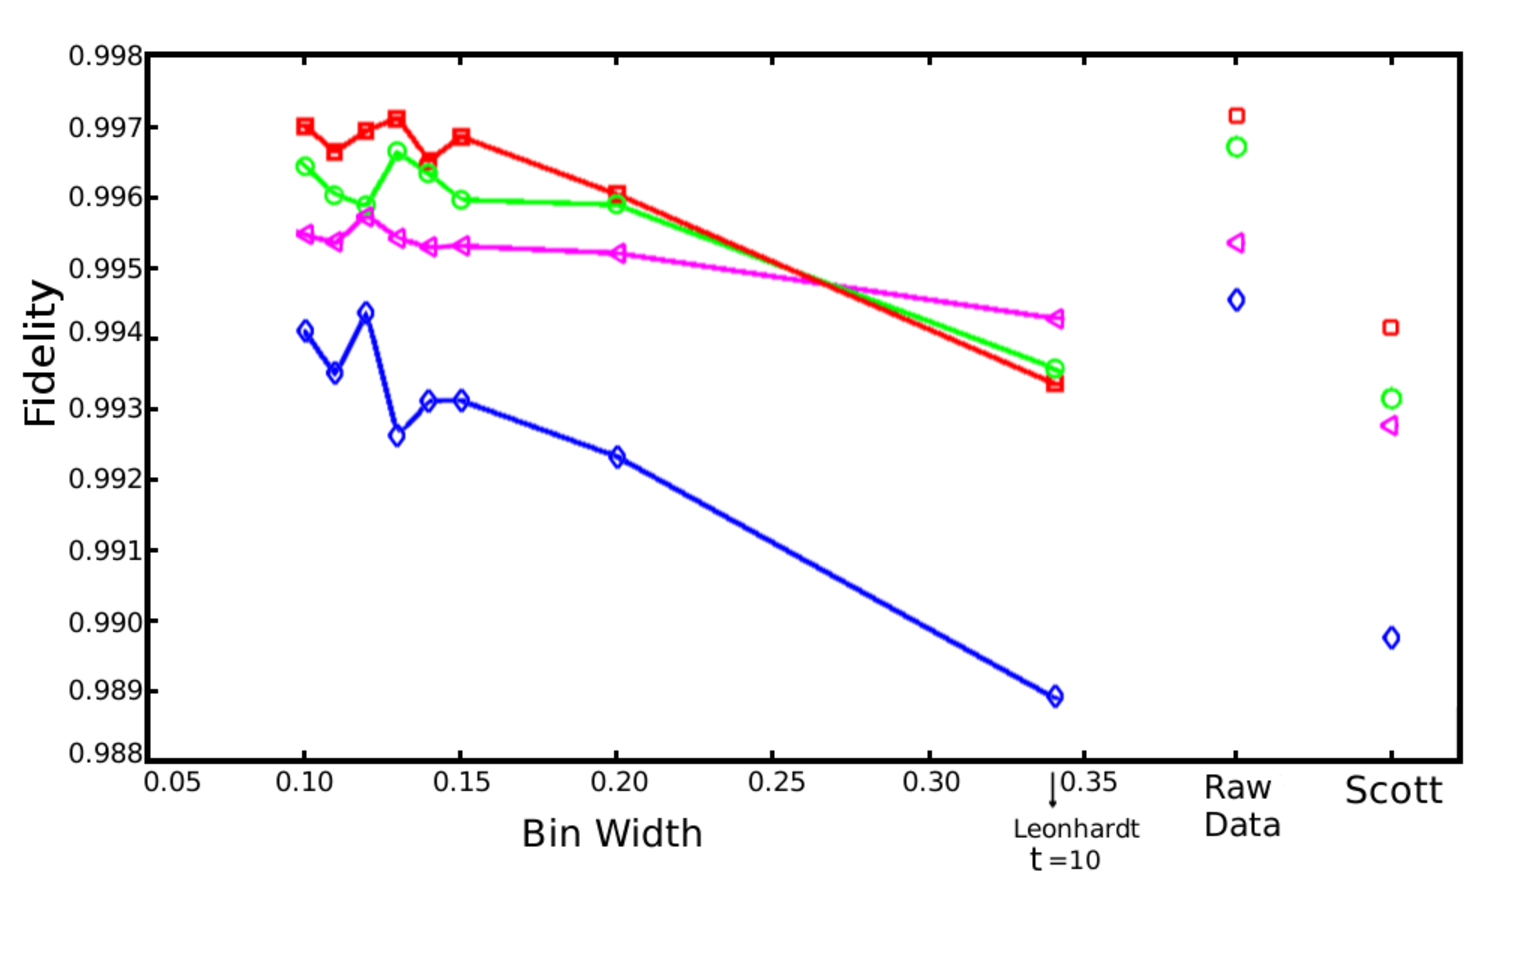
\includegraphics[width=0.5\textwidth]{methods_fidelity_singledata.eps}
\caption{Fidelity as a function of the bin width for a cat state with amplitude $\alpha=1$. The Hilbert space is truncated at 10 photons. Each set of points corresponds to a different data set. The mean bin width for Scott
method is $0.35$.}
\label{fig-methods_fidelity_singledata}
\end{figure}

%DISCUSSION OF FIGURE 2
%In Fig.~

%FIGURA 2
%\begin{figure}[h]
%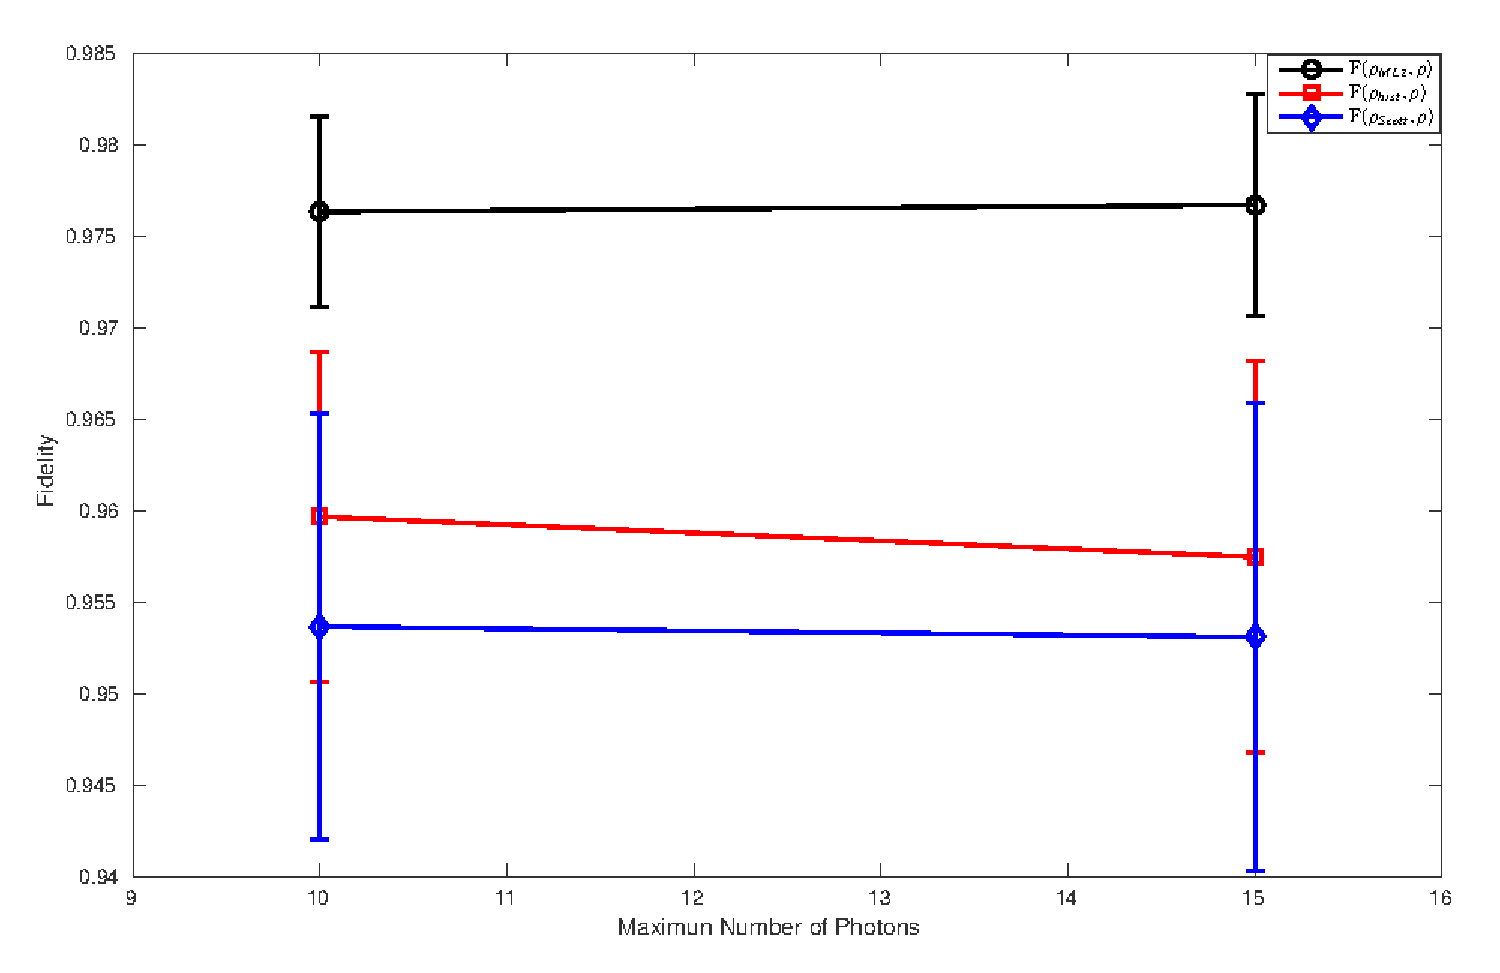
\includegraphics[width=0.49\textwidth]{FockState_(n=5).eps}
%\caption{}
%\label{fig-FockState_(n=5)}
%\end{figure}

%DISCUSSION OF FIGURE 2
The next set of results is presented in Fig.~\ref{fig-fidelity_vs_binwidth_15_photons_catstate}, where we have the fidelity as a function
of the bin width for cat states with amplitudes $\alpha=1$ and $\alpha=2$. The states are reconstructed in a 15 photons Hilbert space. The first thing that we can
notice in this graph is that the fidelity for a $\alpha=1$ cat state is always greater than the fidelity for a $\alpha=2$ cat state, including the case when we
have no binning. This is expected, because a $\alpha = 2$ state requires more parameters to effectively describe its density matrix, so for a given amount of data, there is greater statistical uncertainty. 

We may also notice that the fidelity for the $\alpha = 2$ cat state decreases faster than the fidelity for a $\alpha=1$ cat state as the bin size increases. This is also expected because the $\alpha = 2$ state has more wiggles in its probability distribution, so more information is lost when the bins are larger. The average bin width for Scott method is $0.35$ for a $\alpha=1$ cat state, and $0.64$ for a $\alpha=2$ cat state. 

%FIGURE 2
\begin{figure}[h]
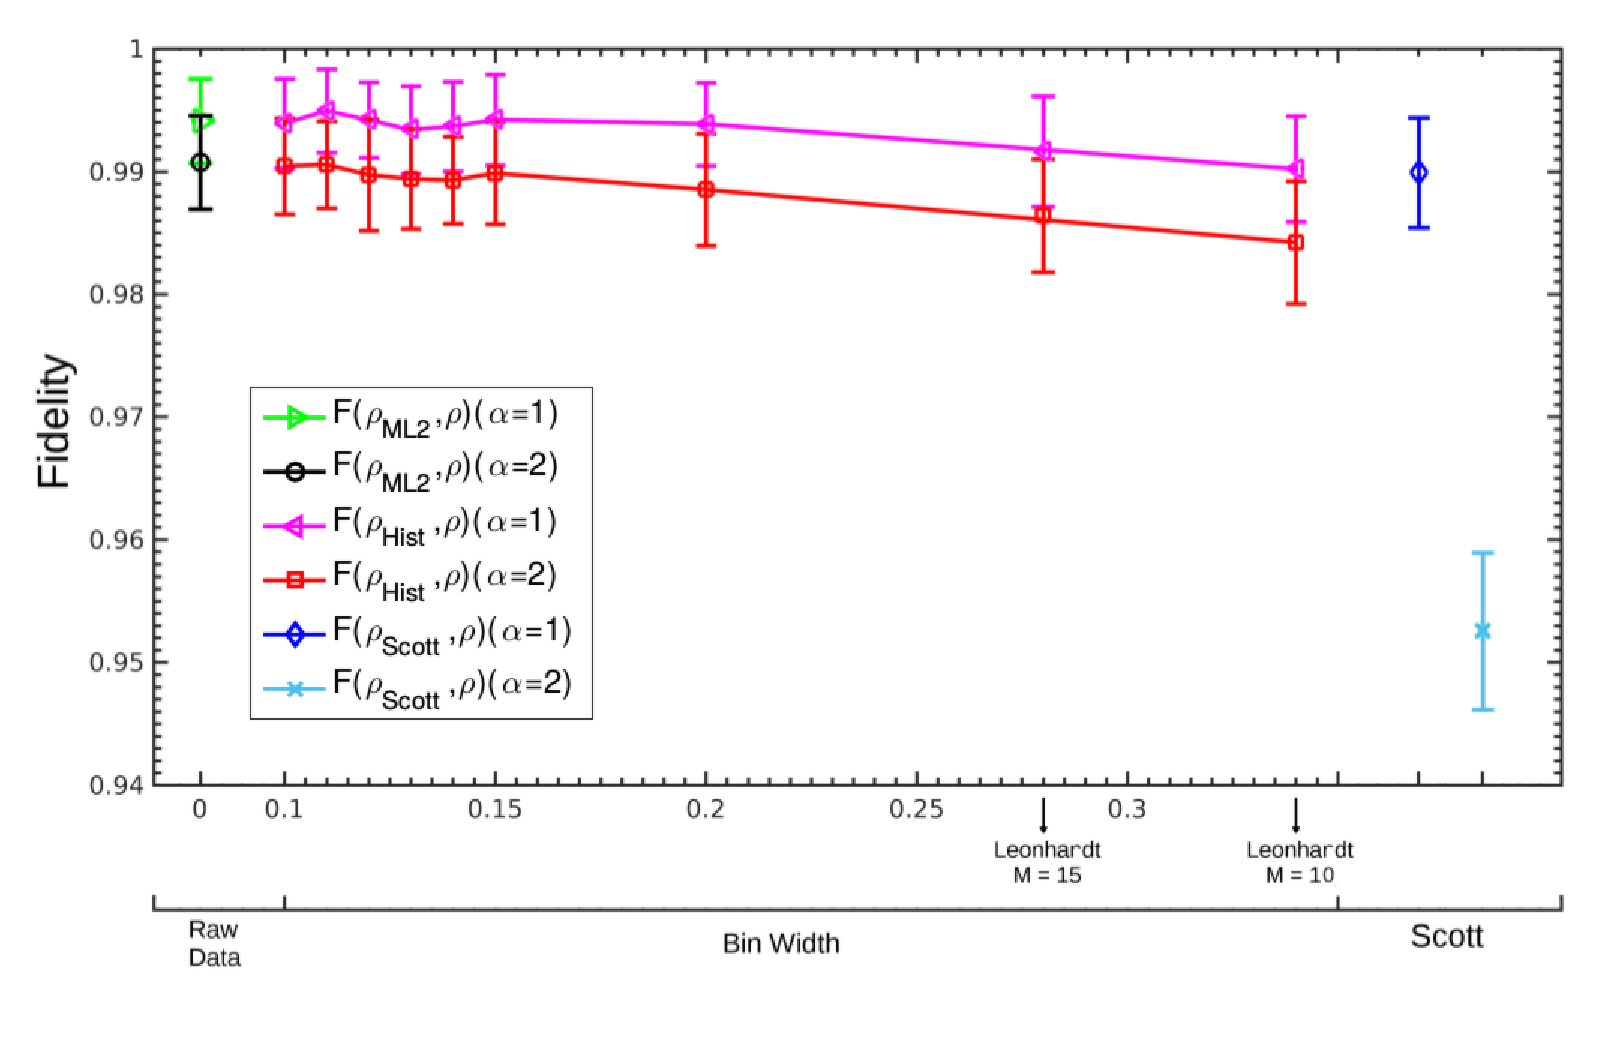
\includegraphics[width=0.49\textwidth]{fidelity_vs_binwidth_15_photons_catstate.eps}
\caption{Fidelity as a function of the bin width for cat states with amplitudes $\alpha=1$ and $\alpha=2$. The Hilbert space is truncated at 15 photons. The mean bin width for Scott method are $0.35$ ($\alpha=1$ cat state) and $0.64$ ($\alpha=2$ cat state).}
\label{fig-fidelity_vs_binwidth_15_photons_catstate}
\end{figure}

%DISCUSSION OF FIGURE 3
Figure~\ref{fig-squeezedvacuum_15_photons_Var=075} shows the fidelity as a function
of the bin width for a squeezed vacuum state whose squeezed quadrature has a variance 3/4 of the vacuum variance.  We use a 15 photon Hilbert space to reconstruct this state. In this graph, we extended the bin width until $1.05$ to help visualize the decreasing in the fidelity when the bin width increases. Using a bin width of $1.05$ gives us a fidelity loss of about $7\%$, while the loss when we use Scott's optimal bin width (0.25) is of about $0.02\%$.

%In Figs.~\ref{fig-fidelity_vs_binwidth_15_photons_catstate} and~\ref{fig-%squeezedvacuum_15_photons_Var=075}, we indicate the bin width obtained using Eq.~(\ref{eq-leonhardt}) for a maximum number of photon in the Hilbert space of $10$ and $15$, respectively. 

%FIGURE 3
\begin{figure}[h]
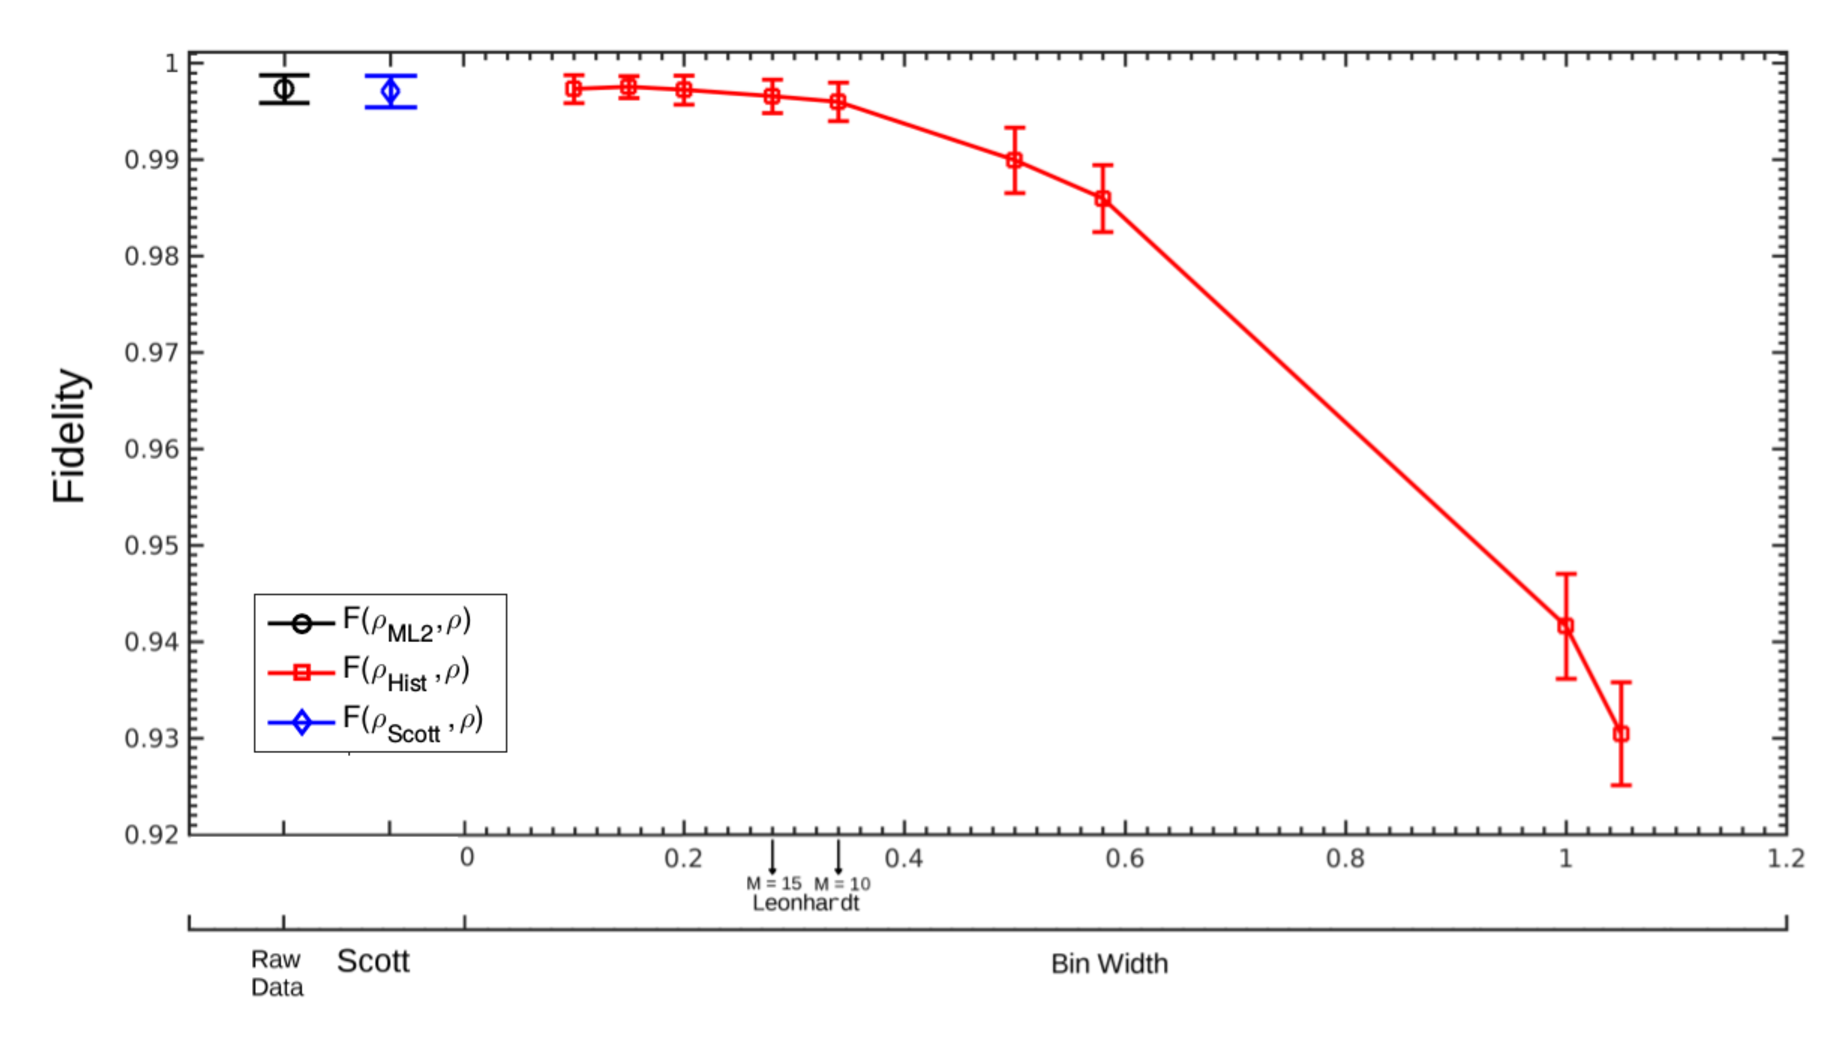
\includegraphics[width=0.49\textwidth]{squeezedvacuum_15_photons_Var=075.eps}
\caption{Fidelity as a function of the bin width for a squeezed vacuum state whose squeezed quadrature has a variance 3/4 of the vacuum variance. The Hilbert space is truncated at 15 photons. The mean bin width for Scott method is $0.25$.}
\label{fig-squeezedvacuum_15_photons_Var=075}
\end{figure}

%DISCUSSION OF FIGURES 4, 5 AND 6
Until now, as mentioned before, each bin's measurement operator represents a measurement that occurs at the center of the bin. In order to improve our analysis,
we now change each bin's measurement operator so that it represents a measurement that occurs anywhere in the bin, rather than a measurement that happens exactly at the center of the bin. For that, we integrate the measurement operators over the width of each histogram bin. We will identify each case by adding $[$POVM-center$]$ and $[$POVM-integral$]$ to the fidelity identifier.

We also add to our analysis the fidelity calculation when using a bin width given by Leonhardt's formula, Eq.~(\ref{eq-leonhardt}), calculated with the mean photon number estimated by Eq.~(\ref{eq-photon-estimation}). In this case, we compute the fidelity between the true state and the density matrix reconstructed using data binning with a bin width given by Leonhardt formula, $\rho_{\mathrm{Leonhardt}}$. We reminder the reader that Leonhardt suggests that the used bin width should be equal or smaller to the one calculated using Eq.~(\ref{eq-leonhardt}). 

In Figs.~\ref{fig-Fidelity_vs_binwidth_catstate_Mph_10_alpha_1} and
~\ref{fig-Fid_vs_binwidth_catstate_alpha_2_Mph_15}, we have the fidelity
as a function of the bin width for cat states with amplitudes $\alpha=1$ and
$\alpha=2$, respectively. We used a $10$ photon Hilbert space to reconstruct the
$\alpha = 1$ cat state, while the $\alpha = 2$ cat state was reconstructed in a
$15$ photon space. On the other hand, Fig.~\ref{fig-squeezed_vacuum_variance_075_Mph_10} shows the fidelity as a function of the 
bin width for a squeezed vacuum state whose squeezed quadrature has a variance 3/4 of the vacuum variance, with a Hilbert space truncated at 10 photons.

For the $\alpha = 1$ cat state in Fig.~\ref{fig-Fidelity_vs_binwidth_catstate_Mph_10_alpha_1}, the estimated mean number of photons is $0.6109$ (real mean number of photons is $0.6093$), what gives us, by Leonhardt's formula, Eq.~(\ref{eq-leonhardt}), a bin width of $1.05$. As mentioned before, the average bin width for Scott method in this case is $0.35$. For the $\alpha = 2$ cat state in Fig.~\ref{fig-Fid_vs_binwidth_catstate_alpha_2_Mph_15}, the estimated mean number of photons is $3.1983$ (real mean number of photons is $3.1978$), giving a bin width of $0.58$. The average bin width for Scott method is $0.64$ for this state. The squeezed vacuum state of Fig.~\ref{fig-squeezed_vacuum_variance_075_Mph_10} has an estimated mean number of photons of
$0.0162$ (real mean number of photons is $0.0167$), giving a bin width, by Eq.~(\ref{eq-leonhardt}), of $1.54$. The average bin width for Scott method, in this case, is $0.25$.

Analyzing the graphs shown in Figs.~\ref{fig-Fidelity_vs_binwidth_catstate_Mph_10_alpha_1}-\ref{fig-squeezed_vacuum_variance_075_Mph_10}, we see that integrating the measurement operators over the width of each histogram bin improves considerably the fidelity for all the cases. We can also see that, for this case, Leonhardt's suggestion can be safely considered an upper bound for the bin width. The two methods considered here, Leonhardt and Scott methods, give faster fidelity estimates with no significant loss of information.
   
%FIGURE 4
\begin{figure}[h]
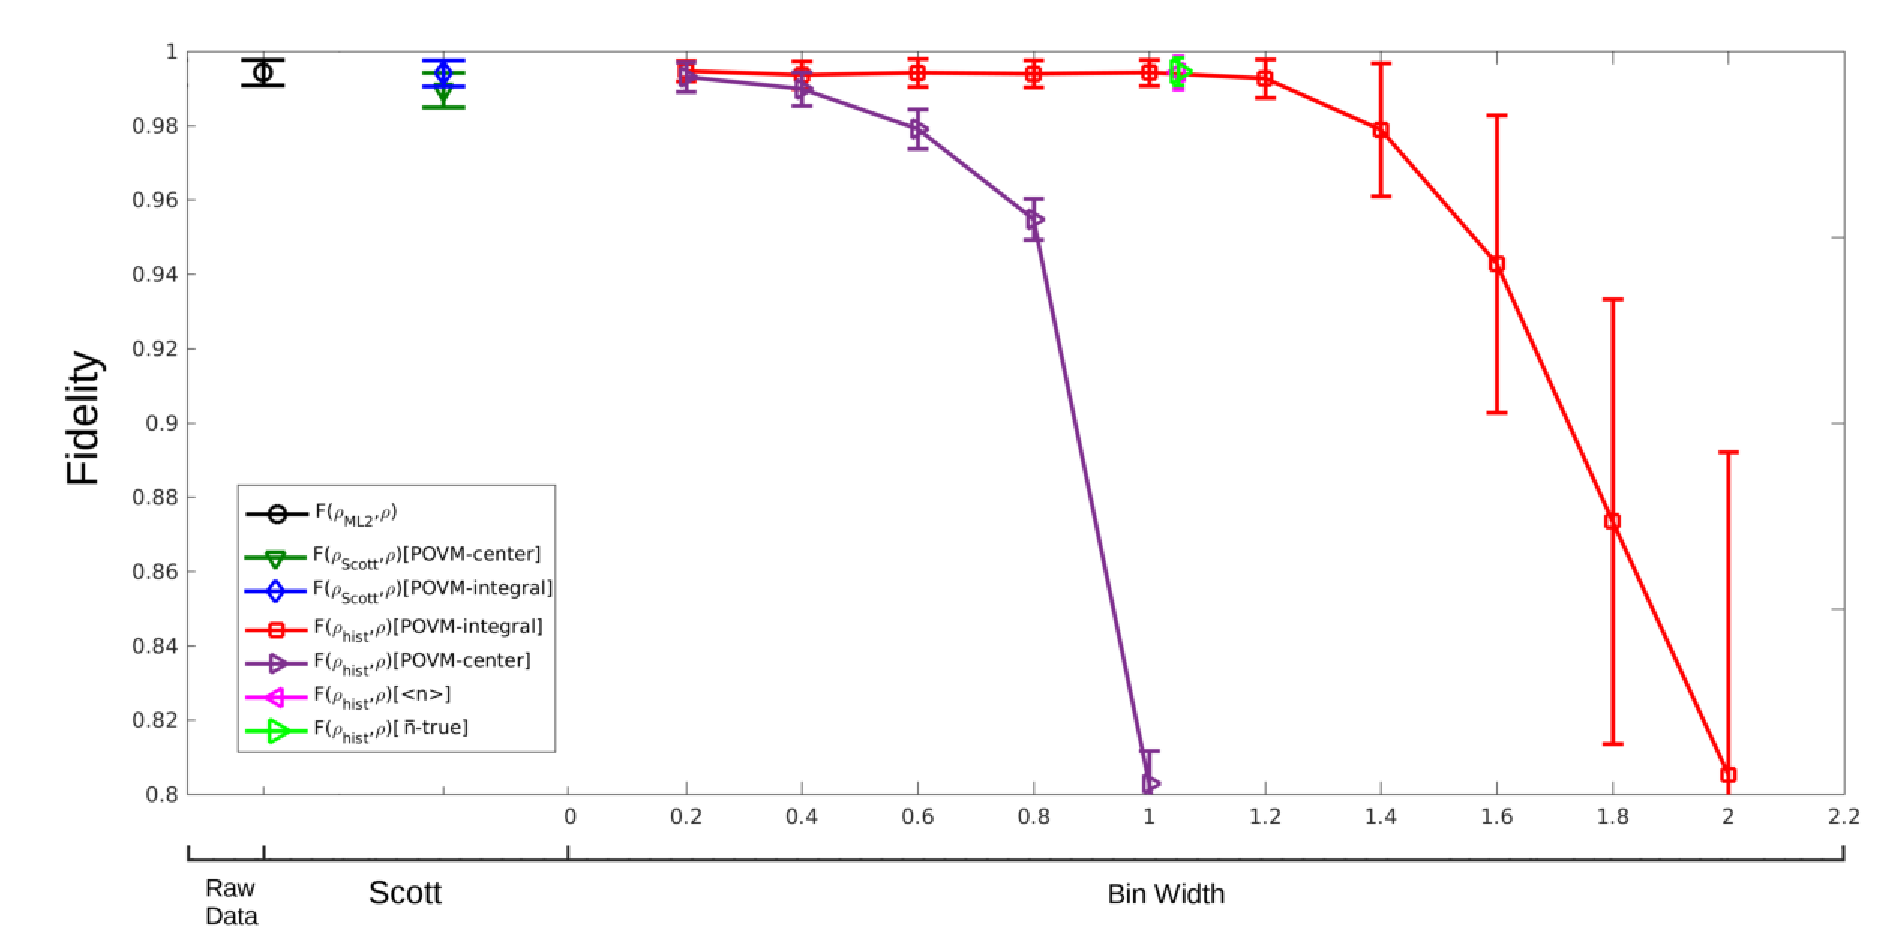
\includegraphics[width=0.49\textwidth]{fid_vs_binwidth_catstate_alpha_1_mph_10.eps}
\caption{Fidelity as a function of the bin width for a cat state with amplitude
$\alpha = 1$. The Hilbert space is truncated at 10 photons. The mean bin width for Scott method is $0.35$, and the bin width given by Leonhardt formula is $1.05$.}
\label{fig-Fidelity_vs_binwidth_catstate_Mph_10_alpha_1}
\end{figure}

%FIGURE 5
\begin{figure}[h]
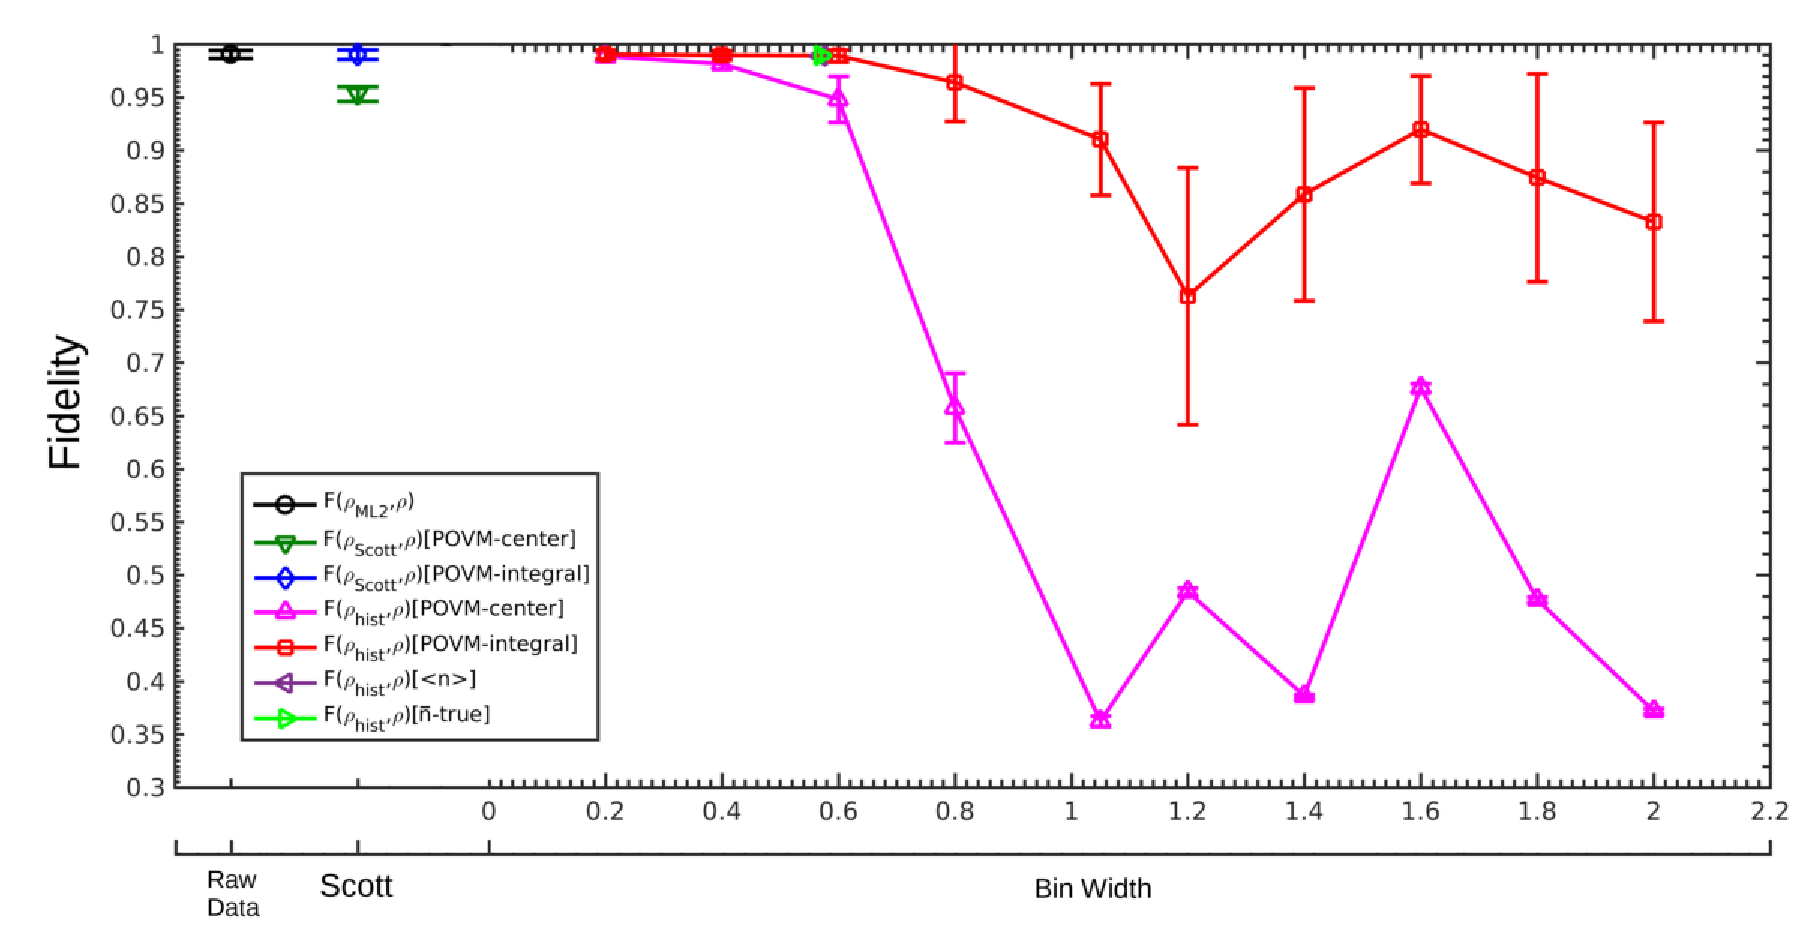
\includegraphics[width=0.49\textwidth]{fidelity_vs_binwidth_catstate_alpha_2.eps}
\caption{Fidelity as a function of the bin width for a cat state with amplitude
$\alpha = 2$. The Hilbert space is truncated at 15 photons. The mean bin width for Scott method is $0.64$, and the bin width given by Leonhardt formula is $0.58$.}
\label{fig-Fid_vs_binwidth_catstate_alpha_2_Mph_15}
\end{figure}

%FIGURE 6
\begin{figure}[h]
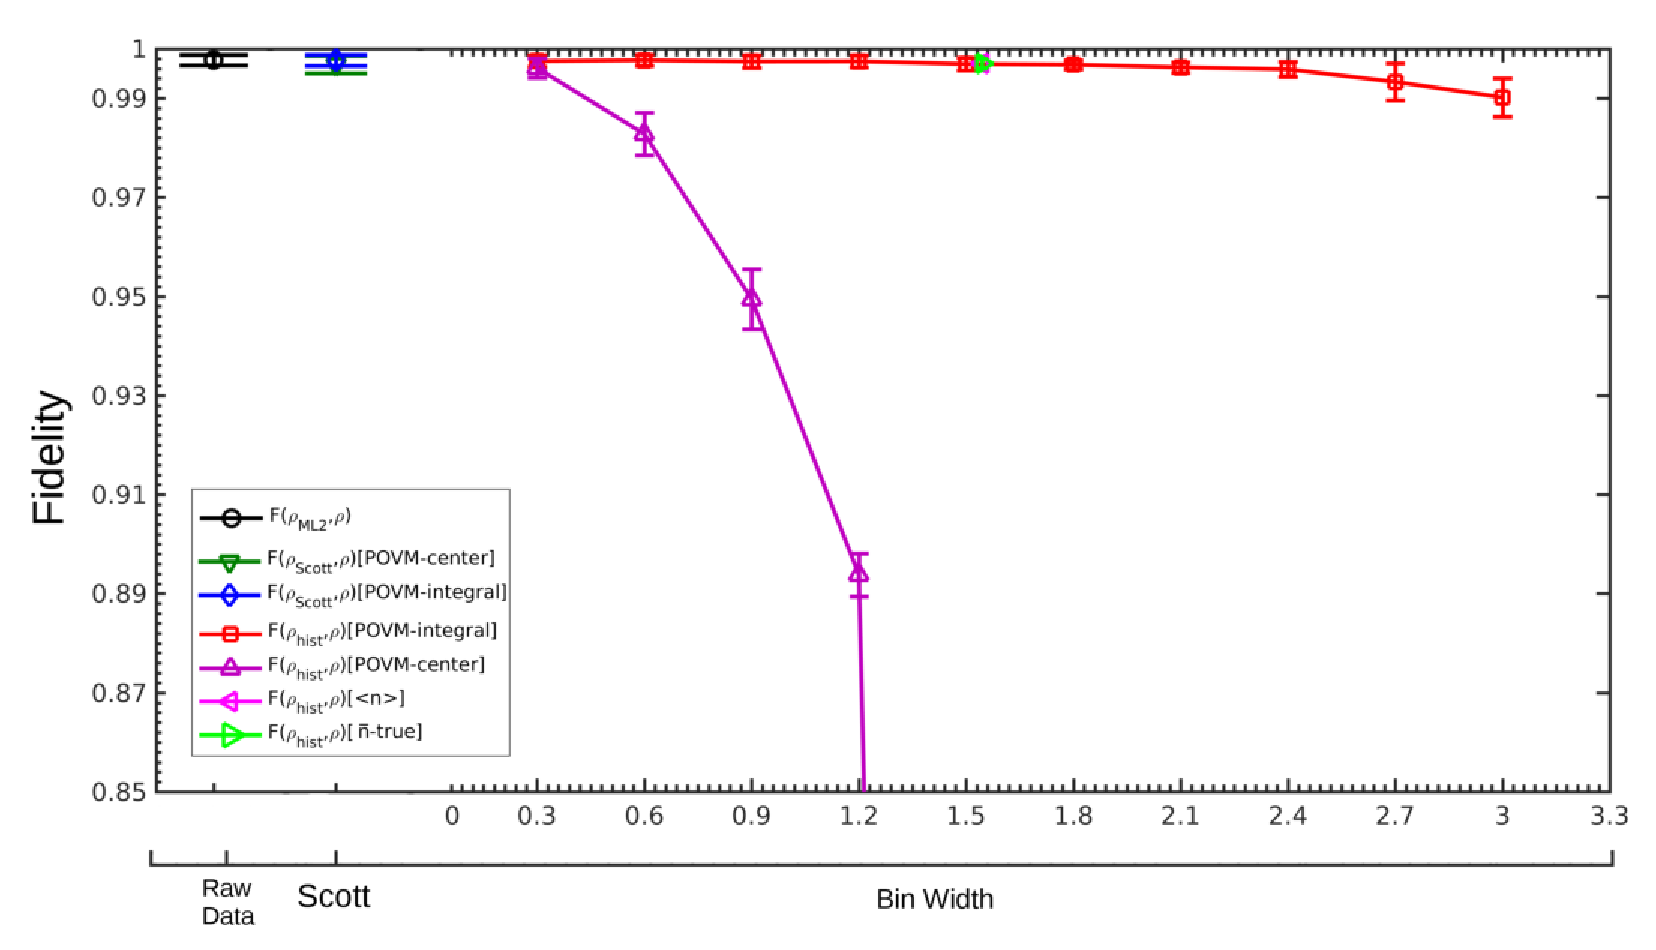
\includegraphics[width=0.49\textwidth]{squeezed_vacuum_variance_075_Mph_10.eps}
\caption{Fidelity as a function of the bin width for a squeezed vacuum state whose squeezed quadrature has a variance 3/4 of the vacuum variance. The Hilbert space is truncated at 10 photons. The mean bin width for Scott method is $0.25$, and the bin width given by Leonhardt formula is $1.54$.}
\label{fig-squeezed_vacuum_variance_075_Mph_10}
\end{figure}

\section{Conclusion}
\label{conclusion}

We have used idealized numerical experiments to generate simulated
data, performed tomography on the data with and without binning, and estimated the fidelity between the reconstructed state and the true state. We used two different
methods to choose the bin width: Scott and Leonhardt methods. We considered the bin’s measurement operator to represent a measurement that occurs at the center of the bin or anywhere in the bin. Our study has focused on maximum likelihood tomography of cat states and squeezed vacuum states. 

Scott method calculates an optimal bin width, for each phase, based on the size and
the standard deviation of the sample. Leonhardt states that we need a bin width
narrower than $q_n/2$, where $q_n$ depends on the number of photons in the state
being reconstructed. Since, in a real experiment, we may not know the mean number
of photons in the state considered, we have proposed a method to determine the 
mean photon number from the quadrature measurement results.    

We have found that our proposed method to find the mean number of photons from the quadrature measurement results gives accurate results. We checked that by comparing
the estimated mean number of photons with the real mean number of photons for the
known states we considered: cat states and squeezed vacuum states. We also have found that integrating the measurement operators over the width of each histogram bin improves significantly the fidelity. Using this strategy, Leonhardt formula safely establishes an upper bound to the bin width, and both methods provides a faster statistical estimation without losing too much information. 



\begin{acknowledgments}
We thank Kevin Coakley, Adam Keith, and Emanuel Knill for helpful
comments on the manuscript.  H. M. Vasconcelos thanks the Schlumberger 
Foundation's Faculty for the Future program for financial support. J. L. E. Silva thanks Coordena\c c\~ao de Aperfei\c coamento de Pessoal de N\'ivel Superior (CAPES) for financial support. This work includes contributions of the National Institute of Standards and
Technology, which are not subject to U.S. copyright.
\end{acknowledgments}


% BibTeX users please use one of
%\bibliographystyle{spbasic}      % basic style, author-year citations
%\bibliographystyle{spmpsci}      % mathematics and physical sciences
%\bibliographystyle{spphys}       % APS-like style for physics
% Scott: My LaTeX does not know about spphys, but it is not necessary
% to specify a bibliography style.  revtex should authomatically use
% the correct style based on the documentclass.
\bibliography{histogram}   % name your BibTeX data base


% Non-BibTeX users please use%\begin{thebibliography}{}
%
% and use \bibitem to create references. Consult the Instructions
% for authors for reference list style.


%\end{thebibliography}


\end{document}

%
% ****** End of file apssamp.tex ******

%%% Local Variables:
%%% mode: latex
%%% TeX-master: t
%%% End:
